% A LaTeX (non-official) template for ISAE projects reports
% Copyright (C) 2014 Damien Roque
% Version: 0.2
% Author: Damien Roque <damien.roque_AT_isae.fr>

\documentclass[a4paper,12pt,calibri,oneside,openany]{book}
\usepackage{geometry}
\usepackage[utf8]{inputenc}
\usepackage[T1]{fontenc}
%\usepackage[french]{babel} % If you write in French
\usepackage[english]{babel} % If you write in English
\usepackage{a4wide}
\usepackage{graphicx}
\graphicspath{{images/}}
\usepackage{subfig}
\usepackage{tikz}
\usetikzlibrary{shapes,arrows}
\usepackage{pgfplots}
\pgfplotsset{compat=newest}
\pgfplotsset{plot coordinates/math parser=false}
\newlength\figureheight
\newlength\figurewidth
\pgfkeys{/pgf/number format/.cd,
set decimal separator={,\!},
1000 sep={\,},
}
\usepackage{ifthen}
\usepackage{ifpdf}
\usepackage{pdfpages}
\ifpdf
\usepackage[pdftex]{hyperref}
\else
\usepackage{hyperref}
\fi
\usepackage{color}
\hypersetup{%
colorlinks=true,
linkcolor=black,
citecolor=black,
urlcolor=black}
\usepackage{float}
\renewcommand{\baselinestretch}{1.05}
\usepackage{fancyhdr}
\pagestyle{fancy}
\fancyfoot{}
\fancyhead[LE,RO]{\textbf{Page \thepage/\pageref{LastPage}}}
\fancyhead[RE]{\bfseries\nouppercase{\leftmark}}
\fancyhead[LO]{\bfseries\nouppercase{\rightmark}}
\setlength{\headheight}{15pt}

\let\headruleORIG\headrule
\renewcommand{\headrule}{\color{black} \headruleORIG}
\renewcommand{\headrulewidth}{1.0pt}
\usepackage{colortbl}
\arrayrulecolor{black}


\usepackage{lastpage}
\renewcommand\headrulewidth{1pt}
\fancyfoot[L]{DMSP}
\renewcommand\footrulewidth{1pt}
\fancyfoot[C]{GREDER Project}
\fancyfoot[R]{\today}
\makeatletter
\def\@textbottom{\vskip \z@ \@plus 1pt}
\let\@texttop\relax
\makeatother

\makeatletter
\def\cleardoublepage{\clearpage\if@twoside \ifodd\c@page\else%
  \hbox{}%
  \thispagestyle{empty}%
  \newpage%
  \if@twocolumn\hbox{}\newpage\fi\fi\fi}
\makeatother

\usepackage{amsthm}
\usepackage{amssymb,amsmath,bbm}
\usepackage{array}
\usepackage{bm}
\usepackage{multirow}
\usepackage[footnote]{acronym}
\usepackage{float}
\usepackage{wasysym}
\usepackage{wrapfig}
\usepackage{url}
\usepackage{eurosym}
\usepackage{array}
\usepackage{xcolor}
\usepackage{supertabular}
%\usepackage{geometry}
\usepackage{pdflscape}
\usepackage{calrsfs}
\usepackage{longtable, booktabs}
\usepackage{minted}
\newcommand*{\SET}[1]  {\ensuremath{\mathbf{#1}}}
\newcommand*{\VEC}[1]  {\ensuremath{\boldsymbol{#1}}}
\newcommand*{\FAM}[1]  {\ensuremath{\boldsymbol{#1}}}
\newcommand*{\MAT}[1]  {\ensuremath{\boldsymbol{#1}}}
\newcommand*{\OP}[1]  {\ensuremath{\mathrm{#1}}}
\newcommand*{\NORM}[1]  {\ensuremath{\left\|#1\right\|}}
\newcommand*{\DPR}[2]  {\ensuremath{\left \langle #1,#2 \right \rangle}}
\newcommand*{\calbf}[1]  {\ensuremath{\boldsymbol{\mathcal{#1}}}}
\newcommand*{\shift}[1]  {\ensuremath{\boldsymbol{#1}}}

\newcommand{\eqdef}{\stackrel{\mathrm{def}}{=}}
\newcommand{\argmax}{\operatornamewithlimits{argmax}}
\newcommand{\argmin}{\operatornamewithlimits{argmin}}
\newcommand{\ud}{\, \mathrm{d}}
\newcommand{\vect}{\text{Vect}}
\newcommand{\sinc}{\ensuremath{\mathrm{sinc}}}
\newcommand{\esp}{\ensuremath{\mathbb{E}}}
\newcommand{\hilbert}{\ensuremath{\mathcal{H}}}
\newcommand{\fourier}{\ensuremath{\mathcal{F}}}
\newcommand{\sgn}{\text{sgn}}
\newcommand{\intTT}{\int_{-T}^{T}}
\newcommand{\intT}{\int_{-\frac{T}{2}}^{\frac{T}{2}}}
\newcommand{\intinf}{\int_{-\infty}^{+\infty}}
\newcommand{\Sh}{\ensuremath{\boldsymbol{S}}}
\newcommand{\C}{\SET{C}}
\newcommand{\R}{\SET{R}}
\newcommand{\Z}{\SET{Z}}
\newcommand{\N}{\SET{N}}
\newcommand{\K}{\SET{K}}
\newcommand{\reel}{\mathcal{R}}
\newcommand{\imag}{\mathcal{I}}
\newcommand{\cmnr}{c_{m,n}^\reel}
\newcommand{\cmni}{c_{m,n}^\imag}
\newcommand{\cnr}{c_{n}^\reel}
\newcommand{\cni}{c_{n}^\imag}
\newcommand{\tproto}{g}
\newcommand{\rproto}{\check{g}}
\newcommand{\LR}{\mathcal{L}_2(\SET{R})}
\newcommand{\LZ}{\ell_2(\SET{Z})}
\newcommand{\LZI}[1]{\ell_2(\SET{#1})}
\newcommand{\LZZ}{\ell_2(\SET{Z}^2)}
\newcommand{\diag}{\operatorname{diag}}
\newcommand{\noise}{z}
\newcommand{\Noise}{Z}
\newcommand{\filtnoise}{\zeta}
\newcommand{\tp}{g}
\newcommand{\rp}{\check{g}}
\newcommand{\TP}{G}
\newcommand{\RP}{\check{G}}
\newcommand{\dmin}{d_{\mathrm{min}}}
\newcommand{\Dmin}{D_{\mathrm{min}}}
\newcommand{\Image}{\ensuremath{\text{Im}}}
\newcommand{\Span}{\ensuremath{\text{Span}}}

\newcommand{\anfr}[1]{{\bfseries\underline{#1}}}

\newtheoremstyle{break}
  {11pt}{11pt}%
  {\itshape}{}%
  {\bfseries}{}%
  {\newline}{}%
\theoremstyle{break}

%\theoremstyle{definition}
\newtheorem{definition}{Définition}[chapter]

%\theoremstyle{definition}
\newtheorem{theoreme}{Théorème}[chapter]

%\theoremstyle{remark}
\newtheorem{remarque}{Remarque}[chapter]

%\theoremstyle{plain}
\newtheorem{propriete}{Propriété}[chapter]
\newtheorem{exemple}{Exemple}[chapter]



%\sloppy
\usepackage{wrapfig}
\usepackage{enumitem}
\usepackage{pifont}
\usepackage{makeidx}
\usepackage{setspace}
\usepackage{xr}
\usepackage{zref}
\usepackage{zref-xr}
\usepackage{xr-hyper}
\makeindex
\usepackage[xindy]{glossaries}
\makeglossaries
%\loadglsentries{glossaire.tex}




\begin{document}

\renewcommand{\bibname}{Bibliographie et Webographie}
%%%%%%%%%%%%%%%%%%
%%% First page %%%
%%%%%%%%%%%%%%%%%%

\begin{titlepage}
\begin{center}


\includegraphics[width=0.5\textwidth]{logohsb}\\[1cm]

%{\large Étudiants ingénieurs en aérospatial}\\[0.5cm]

%{\large DMSP}\\[0.5cm]

% Title
\rule{\linewidth}{0.5mm} \\[0.4cm]
{ \huge  \textbf{GREDER} \\[0.1cm] \textbf{G}reen \textbf{RE}-usable \textbf{DE}bris \textbf{R}emover }
\rule{\linewidth}{0.5mm} \\[1.5cm]
%\vspace{1cm}
\begin{center}
	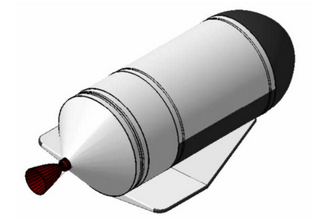
\includegraphics[height=6cm]{greder}
\end{center}
\vspace{0.8cm}
% Author and supervisor
\noindent
\begin{minipage}{0.4\textwidth}
  \begin{flushleft} \large
    \emph{Authors :}\\
    Tim \textbf{\textit{Lewis}}\\
    Alina \textbf{\textit{Trifunovic}}\\
    Lukas \textbf{\textit{Krause}}\\
    Alexis \textbf{\textit{Rolin}}\\
    Julien \textbf{\textit{Huynh}}\
  \end{flushleft}
\end{minipage}%
\begin{minipage}{0.4\textwidth}
  \begin{flushright} \large
    \emph{Supervising professor :} \\
    Prof. Dr.-Ing. Uwe \textit{Apel}\\
  \end{flushright}
\end{minipage}

\vfill

% Bottom of the page
{\large Version 0.7\\ \today}

\end{center}
\end{titlepage}

%%%%%%%%%%%%%%%%%%%%%%%%%%%%%
%%% Non-significant pages %%%
%%%%%%%%%%%%%%%%%%%%%%%%%%%%%

\frontmatter

%\chapter*{Remerciements}


\tableofcontents

\mainmatter
\pagestyle{fancy}
%%%%%%%%%%%%%%%%%%%%%%%%%%%%%%%%%%%%%%%%%%%%
%%% Content of the report and references %%%
%%%%%%%%%%%%%%%%%%%%%%%%%%%%%%%%%%%%%%%%%%%%



\chapter{Introduction}
\chapter{Schedule}

\qquad At the start of the project a dedicated group meeting was performed in order to agree on a common project sequence, tasks and challenges as well as work distribution. This group meeting was deemed essential to structure the work packages and to achieve a consolidated baseline for the whole project including time line.\\

The result is a complex MS project Gantt diagram, which can be found in \nameref{sec:annex1}.\\
\section{Initial Schedule}
\qquad The first version of the schedule starts with a project Kick-Off in October which is afterwards followed by a short planning phase. In this planning phase issues as scheduling, work distribution and scope of the project were addressed.\\

Subsequently, the definition phase started. Within this phase, the vehicle requirements were defined and the mission was planned, calculated and visualized in MATLAB. The outcomes of the definition phase are the boundary requirements which are set to provide a frame for both: the vehicle itself as well as the propulsion system. The requirements were defined at the beginning of the project and were verified after project completion.\\

Upon definition of the boundary requirements, the specification phase started. Within this phase, different propellant combinations were identified, discussed and compared. Additionally a first mass budget was calculated. The result of this phase is the system specification.\\

The sequence of the project includes several presentations. The first one was performed in October for a quick overview on the project planning. The second one after the boundary requirements and system specification was set. 
After this presentation, the vehicle and sub system design phase started. This phase included major parts of the work packages including propulsion system design with all sub-assemblies as RACS/ACS, propellant tanks, feeding and pressurization system, turbo pumps, catalyzer, engine, injector and nozzle. The outcome of this phase is a preliminary vehicle design and sub system design which was presented in the mid-term presentation.\\

As a last major work package the simulation phase started. The whole system was simulated including all sub systems and additionally the complex H2O2 decomposition regulation. The final presentation was performed after all tasks were completed and the simulation was finalized.\\

An overview the compressed initial schedule is shown in \autoref{Fig1}. The detailed Gantt schedule can be found in Annex 1.

\begin{figure}[H]
	\centering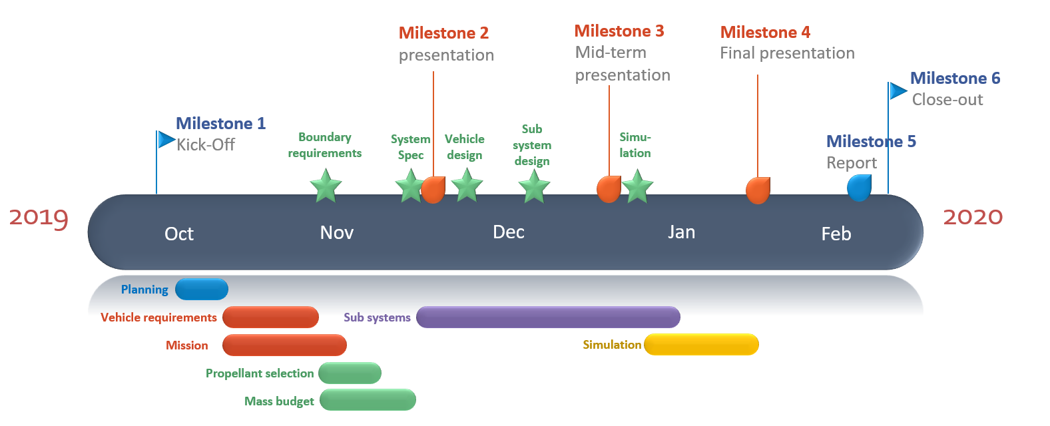
\includegraphics[width=\linewidth]{initialschedule}
	\caption{Initial schedule}\label{Fig1}
\end{figure}

\section{Final schedule – comparison as planned and as achieved}

\qquad As usual in project management and project work, not all milestones were achieved in time. As it is shown in the compressed final schedule in \autoref{Fig2}, the finalized vehicle design, the finalized sub system design and the corresponding simulation shifted within the project schedule (\autoref{Fig2}, shown in red). Nevertheless all work packages have been successfully completed until Milestone 4, the final presentation.

\begin{figure}[H]
	\centering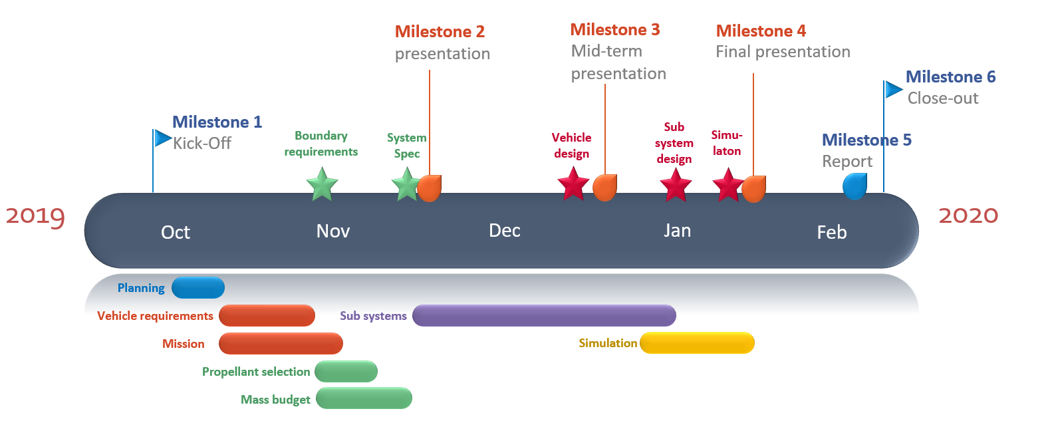
\includegraphics[width=\linewidth]{finalschedule}
	\caption{Final schedule - comparison as planned and as achieved}\label{Fig2}
\end{figure}


\chapter{Requirements}
\qquad The top level requirements for the vehicle and propulsion system are divided in three categories: operation, environment and vehicle. The operation requirements are related to the propulsion system and its applicability for the planned missions. The environmental requirements are defined to ensure that both the vehicle and propulsion system is capable of operating and sustaining during launch, mission and in space environment. The scope of the vehicle requirements is to cover the major parts of the planned mission as refuel-ability, aero braking or accuracy. \\
\noindent
\begin{table}
\begin{tabular}{|c|}
	\hline
	\cellcolor{blue!60}\textbf{Operation}\\
	\hline
	\cellcolor{blue!15} TL-1 Provide sufficient thrust for completion of the mission profile including a safety margin\\
	\hline
	\cellcolor{blue!15} TL-2 Re-ignitable at least 1000 times\\
	\hline
	\cellcolor{blue!15} TL-3 Service life time of at least 100 missions or 25 years in orbit\\
	\hline
	\cellcolor{blue!15} TL-4 Ignition and functional reliability shall be higher than 99,5\%\\

	\hline
	\cellcolor{blue!60}\textbf{Environment}\\
	\hline
	\cellcolor{blue!15} TL-5 Withstand the launch phase
	\\
	\hline
	\cellcolor{blue!15} TL-6 Operate in vacuum
	\\
	\hline
	\cellcolor{blue!15} TL-7 Operate in an ambient temperature range of 1K to 5K
	\\
	\hline
	\cellcolor{blue!15} TL-8 Withstand the temperature gradients resulting from areas turned towards or away
	\\
	\hline
	\cellcolor{blue!15} TL-9 Sustain space-related radiation throughout it's complete life time
	
	\\
	\hline
	\cellcolor{blue!15} TL-10 Withstand debris impact of under 1cm diameter with a max relative speed of $15$ km/s 	
	\\
	\hline
	\cellcolor{blue!60}\textbf{Vehicle}\\
	\hline
	\cellcolor{blue!15} TL-11 The engine shall be the main propulsion system of a GEO satellite recovery vehicle
	\\
	\hline
	\cellcolor{blue!15} TL-12 Refuelable between missions
	\\
	\hline
	\cellcolor{blue!15} TL-13 Perform aerobrake maneuvers in Earth's atmosphere.
	\\
	\hline
	\cellcolor{blue!15} TL-14 Control \space flight path in  Earth's atmosphere  using non-propulsive flight control systems
	\\
	\cellcolor{blue!15} TL-15 Remain within the ARIANE 6/Falcon 9 payload launch capabilities to LEO.
	
	\\
	\cellcolor{blue!15} TL-16 Remain on it's guided trajectory with less than 0.1\% deviation.
	
	\\
	\hline
\end{tabular}
\caption{Requirements for the vehicle}
\end{table}
\chapter{Specification}
\section{Satellite catching process}
\subsection{Choice of the process}

\qquad In order to catch and de-orbit a satellite in GEO, we considered the following usable tools :
\begin{itemize}
	\item Net
	\item Harpoon
	\item Claw
	\item Magnet
\end{itemize}

Other solutions such as towing the satellite or simply removing them from GEO were not considered as they either did not fit our program or would create too much strain on our spacecraft.\\

We then took a closer look at the feasibility of each solution and compared the advantages and disadvantages :
\begin{center}
	\begin{tabular}[H]{|c|c|c|c|}
		\hline
		\textbf{Solution} & \textbf{Advantages} & \textbf{Drawbacks} & \textbf{Feasibility}\\
		\hline
		\textbf{Net} & Cheap, simple, low mass &Slow, hard to handle & Yes (JAXA, ESA)\\
		\hline
		\textbf{Harpoon} & Fairly cheap & Can create more debris& Yes (ESA)\\
		\hline
		\textbf{Claw} & Safer & Mechanical, moving parts& WIP (CleanSpace One)\\
		\hline
		\textbf{Magnet} &Adjustable, no moving parts & Higher mass, needs power& Research State\\
		\hline
	\end{tabular}
\end{center}

As the main focus of our mission is reliability and re-usability, we made the choice of using magnets to catch and hold the satellite we would like to de-orbit.

\subsection{Magnetic solution}
\qquad Even though we decided that we would use magnets, we needed to make sure it was feasible and to lower the drawbacks related to this solution as much as possible. The first precision we need to make is that we will be using electromagnets in order to regulate the intensity of the current in the coil of it, thus, modulating the attraction force so the contact between our spacecraft and the satellite will not be made at high velocity, avoiding damages and space debris creation. \\

Even though it is still at the state of research, we believe that using electromagnets as our catching solution is realistic as both ESA (with ISAE SupAero) and the NASA have been considering and studying this solution since 2017.\\

However, as a matter of complexity, we will have to make assumptions in order to simplify the problem. The objective in this part is to prove that, with assumptions, this solution can be applied to our mission and to find the required energy to both catch and hold the satellite until its release.
\subsubsection{Assumptions}
In our calculations, we assumed that :
\begin{enumerate}
	\item We can consider the magnetic circuit between GREDER and the nozzle of the satellite is a closed one (no air gaps)
	\item About $0.1$\% of the satellite's mass is magnetically operable
	\item Mutual attraction is relatively low compared to the magnetic force
	\item Residuals in the alloy of the magnets' cores are neglectable
\end{enumerate}
\subsection{Sketching and Calculations}
Using the first assumption, we can use the formula for the magnetic force in a magnetic circuit with no air gap :
\begin{equation}
F = \frac{(\mu NI)^2 A}{2\mu_0 L^2}
\end{equation}
With : 
\begin{itemize}
	\item $\mu$ the magnetic permeability of the core of our magnet (determined by the alloy)
	\item $N$ the number of turns of the coil around the core
	\item $I$ the current running through the coil
	\item $A$ the cross section area of the core
	\item $\mu_0$ the magnetic constant
	\item $L$ the length of the mean magnetic circuit
\end{itemize}
In order to have a good balance between thermal properties and magnetic properties we decided to use an alloy made of $90$\% of iron and $10$\% of cobalt for our core. We decided to use this alloy as iron has the best magnetic properties (high relative magnetic permeability) and added cobalt as it has a higher Curie Temperature than iron but has a lower relative magnetic permeability.

In terms of magnet design, we chose to use a squared cross section of $5cm\times 5cm$ for the magnet core and with a length of $15cm$, made of an iron-cobalt alloy and a copper coil around it. We decided to have $135$ turns of the coil around the core with a coil diameter of $1mm$ in order to not have the wire revolutions stuck to each other. We also want to run a current of $10A$ through the coil.\\

\begin{figure}[H]
	\centering
	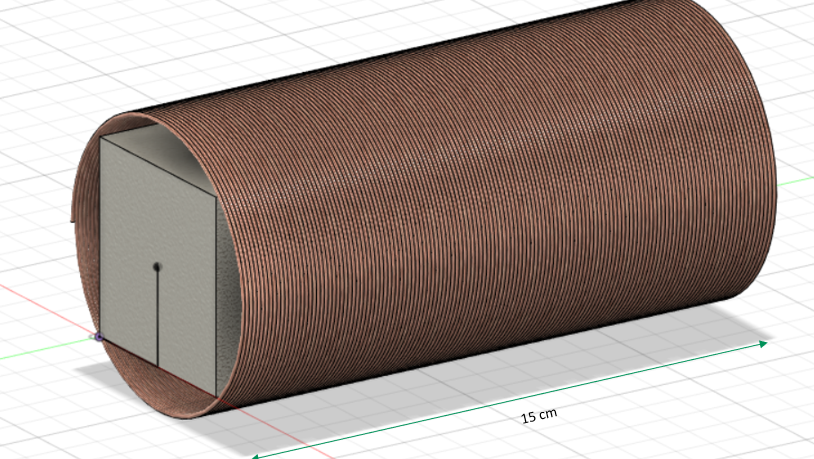
\includegraphics[width=\linewidth]{magnetCAD}
	\caption{CAD of a catching magnet}
\end{figure}


With those design choices we get the following parameters while taking into consideration that there should not be any kind of residuals in the core alloy :

\begin{itemize}
	\item $\mu_0 = 4\pi \times 10^{-7}\ H/m$
	\item $\mu = \bigg(\frac{\mu_{iron}+\mu_{cobalt}}{2}\bigg)\times\mu_0=5.868\times10^{-3}\ H/m$
	\item $N=135$ turns
	\item $I = 10\ A$
	\item $A = 25cm^2=2.5\times10^{-3}\ m^2$
	\item $\rho_{core} = \rho_{iron}\times 0.9 + \rho_{cobalt}\times0.1 = 7.9726\ g/cm^3$
	\item $\rho_{coil} = \rho_{copper} = 8.96\ g/cm^3$
\end{itemize}

We then need to find the length $L$ of the mean magnetic circuit. In order to do so, we decided to start the catching sequence at $10\ m$ from the satellite and that the target has an exploitable nozzle of $40\ cm$ of diameters which is realistic for spacecrafts in the mass range of $3\ 500\ kg$. We could then sketch the catching sequence as so (not to scale) :

\begin{figure}[H]
	\centering
	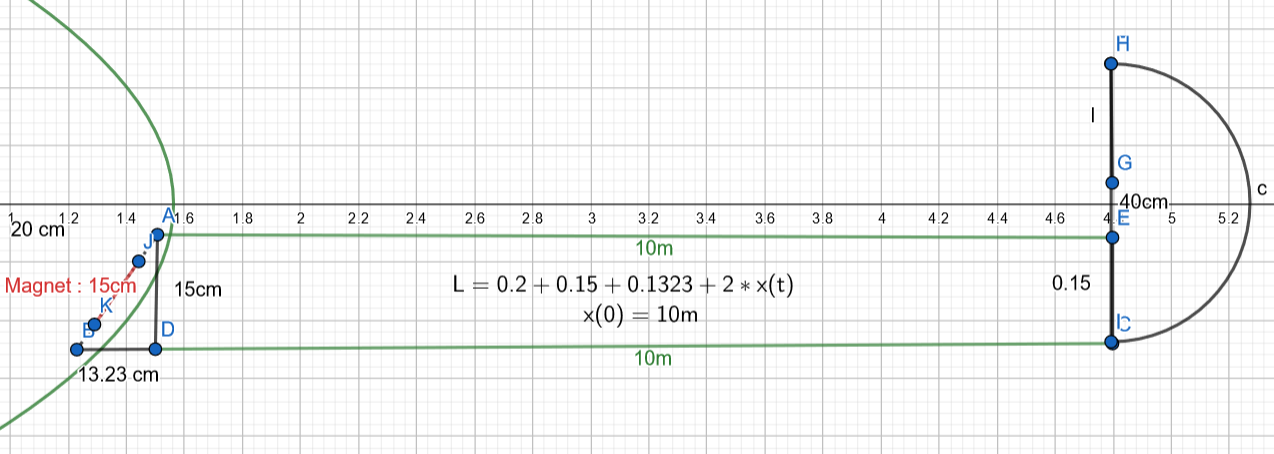
\includegraphics[width=\linewidth]{catching}
	\caption{Catching sequence (not to scale)}
\end{figure}
We can then have the length $L$ as a function of the distance between the tip of our spacecraft and the nozzle of our target. As a result we can proceed to find the feasibility of our solution with this magnet design by finding the time it would require at this state to attract the target. However, in this case, the current modulation when the target is close has not been modeled due to its complexity.\\

Considering that the force will be on one axis only and $m = 0.001\times m_{target} = 3.5\ kg$ :
\begin{align}
\vec F &= m\vec a\\
\frac{(\mu NI)^2 A}{2\mu_0 L(x)^2} &= m \times \ddot x\\
\frac{(\mu NI)^2 A}{2\mu_0 [0.2 + 0.15 + 0.1323 + 2x(t)]^2} &= m \ddot x(t)\\
\frac{(\mu NI)^2 A}{2\mu_0 [0.4823 + 2x(t)]^2} &= m \ddot x(t)
\end{align}

The catching time can then be found using $ode45$ on Matlab :
\begin{minted}[fontsize=\footnotesize, linenos, autogobble, breaklines]{matlab}
clearvars; clc;
catchtime = 1;
x0 = 10;
while 1
[t,x] = ode45(@f3,[0:1:catchtime], [x0; 0; 0; 0]);
if (x(catchtime ,1)>= 2 * x0)
break
else
catchtime = catchtime +1;
end
end
\end{minted}
And the function used for the $ode$ solver :
\begin{minted}[fontsize=\footnotesize, linenos, autogobble, breaklines]{matlab}
function  [Xdot] = f3(t, X)
mu = 5.686e-3; mu0 = 4 * pi * 10 ^(-7);
N = 135; I = 10; A = 0.05 ^ 2; m = 3500 ;
x = X(1); y = X(2); vx = X(3); vy = X(4);
Fmag = (mu * N * I) ^2 * A / (2 * mu0 *(2 * norm(X(1:2)) + 0.4823) ^ 2 );
Xdot = [vx; vy;  0.001 * Fmag / m; 0]; 
end
\end{minted}
We then get a catching time of $812$ seconds. As a result, we can determine the energy required to operate the magnets aswell as their masses and volumes. We are considering a holding time for approximately half an hour and we also need to verify that the magnets will be able to hold the target while we are de-orbiting.

\newpage
\section{Propellant selection}
\newpage
\section{Mass analysis}
\newpage
\hypertarget{header-n0}{%
	\section{Mass Budget - First Iteration}\label{header-n0}}

\qquad Before actually going into our mass budget, we wanted to get a reference
idea for the propellant mass so that we would be sure to be able to
achieve our \(\Delta v\). In order to get this, we decided to find a
relation between the usable propellant mass and the mass of the rest as
a ratio. This is then fixed and will also allow us to know roughly how
much propellant we need depending on the dry mass. Let \(m_{UP}\) be the
mass of usable propellant. Moreover, we would be aiming for a total initial mass of roughly $20$ to $25t$ on our last iteration. This first iteration was done with another magnet design, presented in November which consisted in two large discs of $600\ kg$ each and have then been abandoned for the second iteration.

\hypertarget{header-n3}{%
	\subsection{Coefficients \& Masses after steps}\label{header-n3}}

Considering that \(ISP = 295s\) and annotating
\(\frac{m_{UP_i}}{m_{total_i}} = K_i\) with \(i\) the burn number :

\begin{longtable}[]{@{}cccc@{}}
	\toprule
	Step & Required \(\Delta v\) in \(m/s\) & \(K_i\) & Mass after
	step\tabularnewline
	\midrule
	\endhead
	1 & 2802.4 & 0.620 & 0.38 \(m_{initial}\)\tabularnewline
	2 & 1342.2 & 0.371 & 0.239\(m_{initial}\)\tabularnewline
	3 & 522.9 & 0.165 & 0.200\(m_{initial}\)\tabularnewline
	Satellite caught & NA & NA & 0.2\(m_{initial}\) + 3500\tabularnewline
	4 & 1487.8 & 0.402 & 0.1196\(m_{initial}\) + 2093\tabularnewline
	Satellite release & NA & NA & 0.1196\(m_{initial}\) -
	1407\tabularnewline
	5 & 5.3 & 0.002 & 0.1194\(m_{initial}\) - 1404.186\tabularnewline
	6 & 72.4 & 0.0247 &\tabularnewline
	\bottomrule
\end{longtable}

\hypertarget{header-n51}{%
	\subsection{\texorpdfstring{Global equation between \(m_{UP}\) and
			\(m_{initial}\)}{Global equation between m\_\{UP\} and m\_\{initial\}}}\label{header-n51}}

\begin{longtable}[]{@{}ccc@{}}
	\toprule
	Step & \(\frac{m_{UP}}{m_{initial}}\) & Bias due to
	debris\tabularnewline
	\midrule
	\endhead
	1 & 0.620 & 0\tabularnewline
	2 & 0.141 & 0\tabularnewline
	3 & 0.039 & 0\tabularnewline
	4 & 0.0804 & 1407\tabularnewline
	5 & 0.00024 & -2.814\tabularnewline
	6 & 0.00295 & -36.68\tabularnewline
	TOTAL & 0.88359 & +1369.506\tabularnewline
	\bottomrule
\end{longtable}

We then get our general relation between the usable propellant mass and
the initial mass

\[m_{prop} = 0.88359 m_{init} + 1369.506\]

And as \(m_{initial} = m_{UP} + m_{rest}\) :

\[m_{prop} = \frac 1{0.11641}\bigg[0.88359 m_{rest} + 1369.506\bigg]\]

\(m_{rest}\) includes the dry mass and the propellant required for the
ACS.

\hypertarget{header-n90}{%
	\subsection{First iteration of mass budget}\label{header-n90}}

\hypertarget{header-n91}{%
	\subsubsection{Sub systems}\label{header-n91}}

\begin{longtable}[]{@{}cc@{}}
	\toprule
	Contributor & Mass in kg\tabularnewline
	\midrule
	\endhead
	\underline{\textbf{EPS}} & -\tabularnewline
	Fuel cells & 165.6727\tabularnewline
	H2 for fuel cell (tank included) & 10\tabularnewline
	Cables & 20\tabularnewline
	GNC & 5\tabularnewline
	Batteries & 61.3333\tabularnewline
	Actuators (for flaps) & 10\tabularnewline
	Servos & 1\tabularnewline
	\underline{\textbf{On board computer}} & 5\tabularnewline
	\underline{\textbf{Telecommunications}} & 10\tabularnewline
	\underline{\textbf{Thermal control}} & 10\tabularnewline
	\underline{\textbf{ACS/RCS}} & -\tabularnewline
	Reaction wheels & 106\tabularnewline
	ACS (without propellant) & 36.16\tabularnewline
	\underline{\textbf{\emph{Total}}} & 440.166\tabularnewline
	\bottomrule
\end{longtable}

\hypertarget{header-n120}{%
	\subsubsection{Payload}\label{header-n120}}

\begin{longtable}[]{@{}cc@{}}
	\toprule
	Contributor & Mass in kg\tabularnewline
	\midrule
	\endhead
	Magnet & 1200\tabularnewline
	\bottomrule
\end{longtable}

\hypertarget{header-n147}{%
	\subsubsection{Structure}\label{header-n147}}

\begin{longtable}[]{@{}cc@{}}
	\toprule
	Contributor & Mass in kg\tabularnewline
	\midrule
	\endhead
	Hull & 509\tabularnewline
	Wing & 54\tabularnewline
	Engine & 60\tabularnewline
	Engine frame & 51\tabularnewline
	Connectors & 25\tabularnewline
	Tanks & 350\tabularnewline
	Heat shield & 472\tabularnewline
	\underline{\textbf{\emph{Total}}} & 1521\tabularnewline
	\bottomrule
\end{longtable}

\hypertarget{header-n156}{%
	\subsubsection{Others}\label{header-n156}}

\begin{longtable}[]{@{}cc@{}}
	\toprule
	Contributor & Mass in kg\tabularnewline
	\midrule
	\endhead
	Catalyzer & 10\tabularnewline
	Lines & 25\tabularnewline
	ACS including Propellant & 672\tabularnewline
	Non usable propellant (Residuals, transient, etc.) & 200\tabularnewline
	Helium (including tank) & 30\tabularnewline
	\underline{\textbf{\emph{Total}}} & 937\tabularnewline
	\bottomrule
\end{longtable}

We then get

\[m_{rest} = m_{Sub systems} + m_{Payload} + m_{Structure} + m_{Others} = 4098.166kg\]

Which, with the previously obtained equation :

\[m_{UP} = 42\ 870.926kg\\\]

As the mixture ratio is $MR = 7.07$ and $m_{UP} = m_{UF} + m_{UOP}$\\
\begin{align*}
m_{UsableFuel} &= \frac{m_{UP}}{1 + MR} = 5\ 312kg\\
m_{UsableOxidizer} &= MR \times m_{UsableFuel} =37\ 559kg
\end{align*}

\subsubsection{Results}
We can sum this first iteration up with the following table :
\begin{center}
	\begin{tabular}[H]{|c|c|}
		\hline
		\cellcolor{gray!50}\textbf{Contributor} & \cellcolor{green!20}\textbf{Mass} (kg)\\
		\hline
		\textbf{Structure} & $1\ 521$\\
		\hline
		\textbf{Magnets} & $1\ 200$\\
		\hline
		\textbf{Sub Systems} & $440.166$\\
		\hline
		\textbf{Tank Pressurization} & $30$\\
		\hline
		\textbf{Engine} & $60$\\
		\hline
		\textbf{Catalyzer} & $10$\\
		\hline
		\textbf{Lines} & $25$\\
		\hline
		\cellcolor{gray!50}\textbf{Dry mass} & \cellcolor{green!20} $3\ 286.166$\\
		\hline
		\textbf{Non usable propellant} & $200$\\
		\hline
		\textbf{ACS/RCS Propellant} & $142. 12$\\
		\hline
		\textbf{Usable propellant} & $42\ 870.926$\\
		\cellcolor{red!50}\textbf{Total initial mass} & \cellcolor{red!50}$46\ 969.092$\\
		\hline 
	\end{tabular}
\end{center}
This first initial mass is way over what we are targeting and there are many parameters to be refined during the next iteration.
\newpage
\section{Mass Budget - Second iteration}
\qquad After refining multiple parameters and fixing others to get more accurate values, we went into the second iteration of our mass budget. Having our $I_{SP}$ changed also required another iteration in our calculation formula between the usable propellant mass the the rest of the mass.
\hypertarget{header-n422}{%
	\subsection{Coefficients \& Masses after steps}\label{header-n422}}

Considering that \(ISP = 315s\) and annotating
\(\frac{m_{UP_i}}{m_{total_i}} = K_i\) with \(i\) the burn number :

\begin{longtable}[]{@{}cccc@{}}
	\toprule
	Step & Required \(\Delta v\) in \(m/s\) & \(K_i\) & Mass after
	step\tabularnewline
	\midrule
	\endhead
	1 & 2802.4 & 0.596 & 0.404 \(m_{initial}\)\tabularnewline
	2 & 1342.2 & 0.352 & 0.261792\(m_{initial}\)\tabularnewline
	3 & 522.9 & 0.156 & 0.221\(m_{initial}\)\tabularnewline
	Satellite caught & NA & NA & 0.221\(m_{initial}\) + 3500\tabularnewline
	4 & 1487.8 & 0.382 & 0.137\(m_{initial}\) + 2163\tabularnewline
	Satellite release & NA & NA & 0.137\(m_{initial}\) -1337\tabularnewline
	5 & 5.3 & 0.0017 & 0.1368\(m_{initial}\) - 1334.73\tabularnewline
	6 & 72.4 & 0.023 &\tabularnewline
	\bottomrule
\end{longtable}

\hypertarget{header-n470}{%
	\subsection{\texorpdfstring{Global equation between \(m_{UP}\) and
			\(m_{initial}\)}{Global equation between m\_\{UP\} and m\_\{initial\}}}\label{header-n470}}

Here, we are calculating the percentage of the initial mass that is
required in terms of usable propellant to do each step and then summing
it up to get the percentage of usable mass compared to the total mass to
complete the mission in terms of burns.\\


\subsection{Second iteration of mass budget}

\qquad As our way of presenting our first iteration of the mass budget didn't seems clear enough to us, we decided to present it in another, more logical way :
\begin{longtable}[]{@{}ccc@{}}
	\toprule
	Step & \(\frac{m_{UP}}{m_{initial}}\) & Bias due to
	debris\tabularnewline
	\midrule
	\endhead
	1 & 0.596 & 0\tabularnewline
	2 & 0.142 & 0\tabularnewline
	3 & 0.041 & 0\tabularnewline
	4 & 0.084 & 1337\tabularnewline
	5 & 0.0002 & -2.273\tabularnewline
	6 & 0.0032 & -30.699\tabularnewline
	TOTAL & 0.8664 & +1304.028\tabularnewline
	\bottomrule
\end{longtable}

In this second iteration with a better \(I_{sp}\), we gained
approximately \(1.7\)\% in pure usable propellant mass and about \(5\)\%
on the phases were the satellite creates a bias. We could then either
lower our initial mass or allocate what we have saved there to other
systems that may require more mass.\\

\newpage
\section{Frozen information}
After our second iteration of the mass budget, we decided to make a list of the fixed values that we will work around in our further design.
\subsection{Frozen points}
\begin{itemize}
	\item We will do $20$ aerobrakes
	\item We will have a separate tank design
	\item $H_2O_2$ will be pressurized by its decomposition
	\item The decomposition control will be managed by rotation of the spacecraft
	\item ACS/RCS Layout similar to the Space Shuttle
	\item $H_2O_2$ catalyzers separate
	\item $H_2O_2/O_2$ separation via thermodynamic properties
	\item $H_2/O_2$ will be used in fuel cells to produce energy
\end{itemize}
\begin{center}
	\begin{tabular}[H]{|c|c|c|}
		\hline
		\cellcolor{gray!50}Data & \cellcolor{gray!50}Value & \cellcolor{gray!50}Unit\\
		\hline
		Empty raw mass & $2\ 031$ & kg\\
		\hline
		Usable propellant & $22\ 931$ &kg\\
		\hline
		\cellcolor{green!50}Total mass & \cellcolor{green!50}$24\ 962$ & \cellcolor{green!50}kg\\
		\hline
		Flowrate & $10$ & kg/s\\
		\hline
		Rocket diameter & $2$ & $m$\\
		\hline
		$I_{sp_{vacuum}}$ & $335$ & s\\
		\hline
		Thrust $F=\dot m I_{sp} g_0$ & $32 863.5$ &N\\
		\hline
		Mixture Ratio & $7.07$ & -\\
		\hline
		Wall thickness & $TBA$ & m\\
		\hline
		$H_2O_2$ internal pressure & $1.35$ & bar\\
		\hline
	\end{tabular}
\end{center}
\newpage
\section{Mass Budget - Third iteration}
As the fixed $I_{sp}$ has been refined, we went into our third iteration of the mass budget with the same process as the two previous ones.
\subsection{Coefficients \& Masses after steps}

Considering that \(ISP = 335s\) and annotating
\(\frac{m_{UP_i}}{m_{total_i}} = K_i\) with \(i\) the burn number :

\begin{longtable}[]{@{}cccc@{}}
\toprule
Step & Required \(\Delta v\) in \(m/s\) & \(K_i\) & Mass after
step\tabularnewline
\midrule
\endhead
1 & 2802.4 & 0.574 & 0.426 \(m_{initial}\)\tabularnewline
2 & 1342.2 & 0.335 & 0.283\(m_{initial}\)\tabularnewline
3 & 522.9 & 0.148 & 0.241\(m_{initial}\)\tabularnewline
Satellite caught & NA & NA & 0.221\(m_{initial}\) + 3500\tabularnewline
4 & 1487.8 & 0.364 & 0.153\(m_{initial}\) + 2226\tabularnewline
Satellite release & NA & NA & 0.153\(m_{initial}\) -1274\tabularnewline
5 & 5.3 & 0.0016 & 0.1528\(m_{initial}\) - 1271.96\tabularnewline
6 & 72.4 & 0.0218 &\tabularnewline
\bottomrule
\end{longtable}

\hypertarget{header-n470}{%
\subsection{\texorpdfstring{Global equation between \(m_{UP}\) and
		\(m_{initial}\)}{Global equation between m\_\{UP\} and m\_\{initial\}}}\label{header-n470}}



\begin{longtable}[]{@{}ccc@{}}
\toprule
Step & \(\frac{m_{UP}}{m_{initial}}\) & Bias due to
debris\tabularnewline
\midrule
\endhead
1 & 0.574 & 0\tabularnewline
2 & 0.143 & 0\tabularnewline
3 & 0.042 & 0\tabularnewline
4 & 0.088 & 1274\tabularnewline
5 & 0.0002 & 4.186\tabularnewline
6 & 0.0033 & -36.68\tabularnewline
TOTAL & 0.8664 & +1304.028\tabularnewline
\bottomrule
\end{longtable}
\section{Simulation concept}

\chapter{Design of propulsion systems}
\section{System conceptualization}
\section{Subsystem design}
\subsection{Feeding system}
After having designed most of our propulsion system. We need to carefully link them by designing our feeding system. The biggest challenge is to create a system that will both fit in our spacecraft and deliver the right amount of propellant from the tanks to the engine through our different, required other subsystems. 

\subsection{Turbo pumps}
As most of our subsystems have a defined pressure drop due to their specific design, we have made the choice to use this feeding system design with all losses included to then design our turbopumps to have a pressure rise in accordance with our pressure requirements. We chose to go with electrically driven turbo pumps as we have a good amount of electrical power since we use fuel cells in our spacecraft.
\section{Design review}
\chapter{Simulations}
\qquad \underline{By} : Lukas
\label{chap:sim}
\section{Engine performance simulation}
\qquad In order to simulate the engine performance, the largest single burn was simulated. As the initial burn for entering a Geostationary Transfer Orbit would require more than $900$ s of engine burn time due to the large starting mass of the spacecraft, roughly half of this initial burn was simulated. An immediate result of the requirement to limit engine burn time to $900$ s is therefore, that the first burn needs to be split into two burns. The engine simulation aims to determine thrust, acceleration, $\Delta v$ and propellant masses over time. A combined MATLAB$^{\mbox{\scriptsize{\textregistered}}}$  / Simulink$^{\mbox{\scriptsize{\textregistered}}}$  was used, calculating thrust based on following equation:
\begin{equation}
	F = \dot m \times C_F \times C^*\\
\end{equation}

with : 
$$
C^* = \frac{p_c\times A_t}{\dot{m}}
$$

and

$$
C_F = \sqrt{\frac{2\times \kappa^2}{\kappa - 1}\times \bigg(\frac{2}{\kappa + 1}\bigg)\times\bigg[1 - \bigg(\frac{p_e}{p_c}\bigg)^{\frac{\kappa - 1}{\kappa}}\bigg]} + \varepsilon\bigg(\frac{p_e-p_a}{p_c}\bigg)
$$

assuming a constant mass flow rate of $\dot{m} = 10$ kg/s. Considering a constant chamber pressure after initial start-up of $40$ bars and an exit pressure of $3900$ Pa, which was determined using RPA, a steady-state thrust of $33.6$kN was observed, as can be seen in \autoref{fig1}. $\kappa$ was determined using RPA as well and, while varying slightly throughout the engine, assumed as constant to facilitate the simulation.

\begin{figure}[H]
	\centering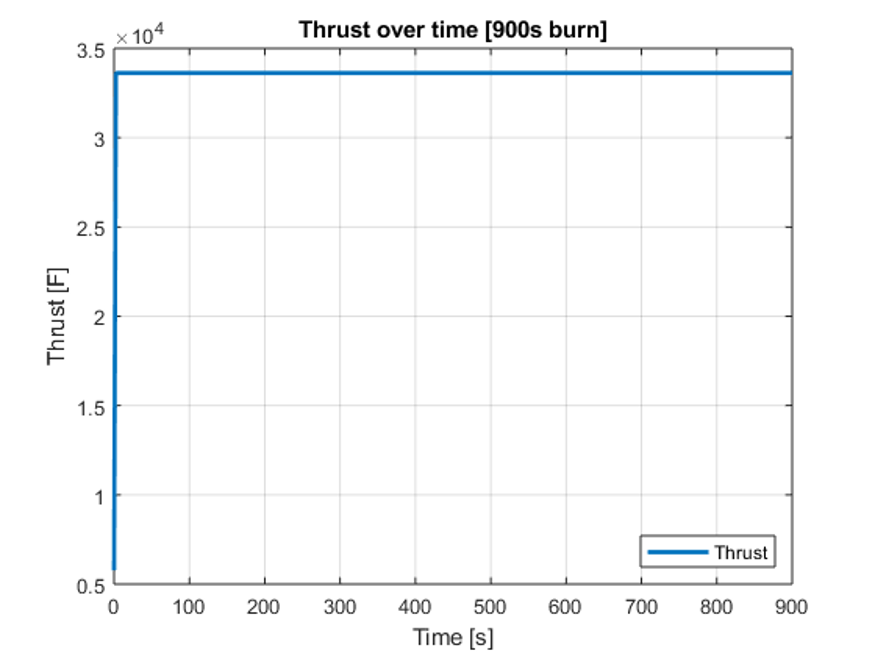
\includegraphics[width=0.9\linewidth]{thrusttime}
	\caption{Engine simulation - Thrust over time}\label{fig1}
\end{figure}

The resulting acceleration and $\Delta v$ over time are shown in \autoref{fig2}.
\begin{figure}[H]
	\centering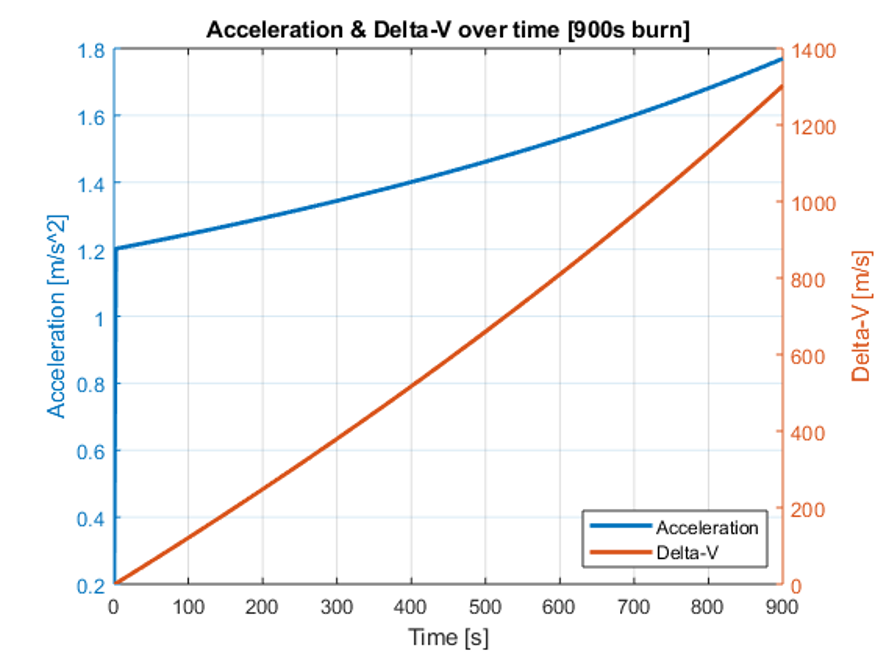
\includegraphics[width=0.9\linewidth]{accdeltav}
	\caption{Engine simulation - Acceleration and $\Delta v$ over time}\label{fig2}
\end{figure}

The acceleration, shown in blue, starts off at around $1.2$ m/s$^2$, which is a value in the range of our expectations. After $900$ seconds, the mass loss leads to a final acceleration of slightly below $1.8$ m/s$^2$, when a $\Delta v$ of ca. $1\ 300$ m/s is reached. At the point of discovery of the insufficiency of $900$ s, the decision to divide the first burn into two was taken. 
Lastly, the behavior of the propellant masses is portrayed in \autoref{fig3}. 

\begin{figure}[H]
	\centering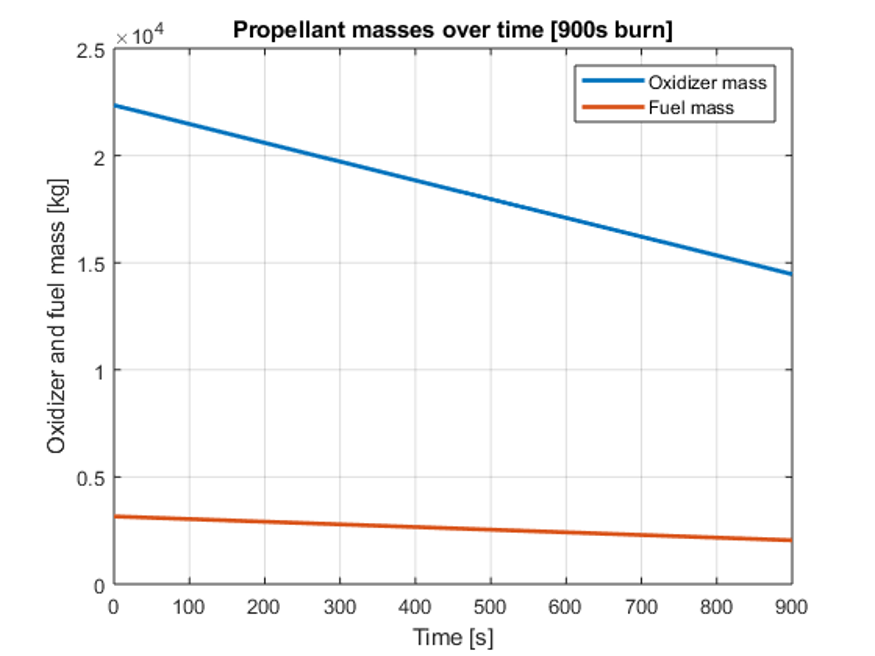
\includegraphics[width=0.9\linewidth]{propmasstime}
	\caption{Engine simulation - Propellant masses over time}\label{fig3}
\end{figure}

With roughly one third of the total usable propellant having been burnt throughout 900 seconds of burn time, these results are also according to expectations. The simulation of the maximum burn time is representative of the entirety of burns throughout the mission, therefore it validates the viability of the engine design for the fulfillment of mission requirements. The complete simulation script and model can be found in the annex. \pagebreak 
\section{Regenerative cooling simulation}

\qquad The thermal loads of the engine combustion are managed by regenerative cooling of the engine, with the cooling channels running along axial lines throughout the entire length of the engine. The cooling liquid is the engine fuel (RP-1), being fed into the combustion chamber wall and running along cooling channels with varying cross-section area before exiting at the end of the nozzle. The cooling channel design was determined by simulation of the relevant wall temperatures in steady-state operation, where a temperature at a given location does not change over time, with heat flux in and out being equal. Following assumptions and design choices were made before and during the preliminary calculations:
\begin{itemize}
	\itemsep0em 
	\item	The inner engine wall is made of copper throughout the entire engine
	\item	The outer wall is made of steel
	\item	A defined number of symmetrical rectangle-shaped cooling channels run through the engine wall, with varying cross-section to allow for higher and lower thermal flux at different sections
	\item	The cooling channels are symmetrical w.r.t. to the engine propellant flow axis
	\item	Injection into the cooling channels takes place at the combustion chamber end of the engine, in order to create larger heat transfer at more thermally stressed areas due to lower coolant temperature
	\item	\textbf{The RP-1 is assumed to not change phase during the regenerative cooling} (While this decreases simulation accuracy, too little data on high-pressure RP-1 phase change behaviour was available. The temperature does however affect the liquid’s heat capacity within the simulation)
\end{itemize}

In order to simulate the steady-state thermal behaviour of the engine along its length, some simplifications needed to be conducted. All coefficients (e.g. ratio of specific heat capacities) are assumed to be constant throughout each section, with three different values for the combustion chamber, throat area and nozzle respectively. In addition, all time-related values were transformed into distance-based values, so that the simulation time is actually millimetres, instead of seconds. This was achieved by limiting the simulation time to the engine length in millimetres and using switches to change constants based on what section the propellant is in at any given millimetre value, while using the flow velocity as the key parameter to transform into metres. The simulation script, model and complete results can be found in the annex. At this point, only some key conclusions will be presented and discussed.\\

The central aim of the iterative calculation was to determine a combination of material, wall thickness and cooling channel geometry which allows the inner wall temperature to remain below its maximum operating temperature. All other temperatures, like the coolant and outer wall temperatures, were of secondary importance. Due to its high thermal conductivity, copper was chosen as the inner wall material.

 The cooling channel cross-section was defined to always be equally sized relative to the local engine diameter, with the ratio being a function of the local engine wall cross-section area and a factor, which represents the filling grade. \autoref{fig4} shows the cross-section change over the engine length. The rectangular geometry is defined by a ratio of width to height of $5$.

\begin{figure}[H]
	\centering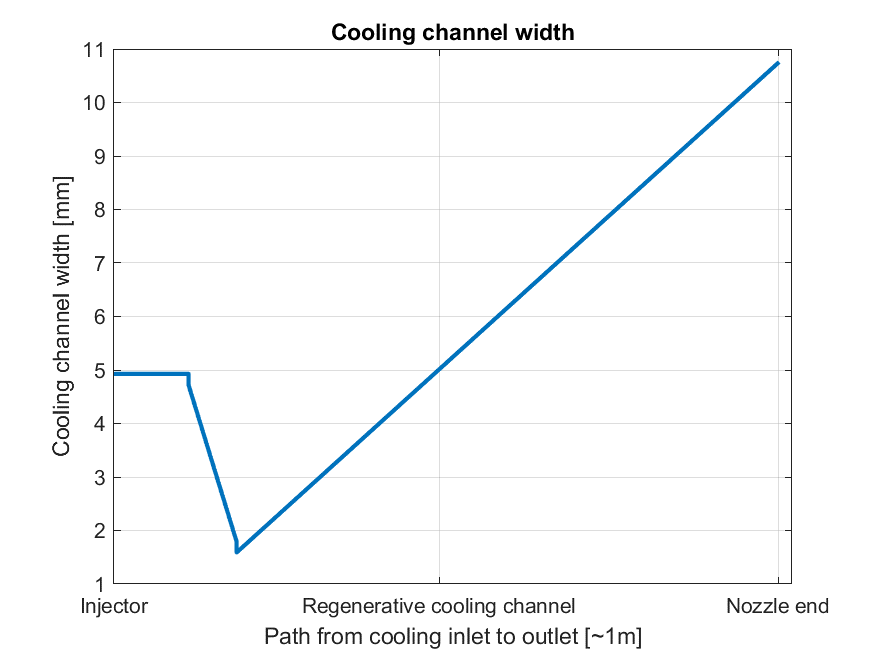
\includegraphics[width=0.9\linewidth]{coolingchannelwidth}
	\caption{Regenerative cooling simulation - Cooling channel width over engine length}\label{fig4}
\end{figure}

The final cooling channel system is a compromise between the copper wall temperature and minimum necessary material for weight savings. Therefore, the copper wall has a thickness of $6$ mm in the combustion chamber, $7$ mm in the throat area and $5$ mm in the nozzle section. The resulting relevant temperatures can be seen in \autoref{fig5}.

\begin{figure}[H]
	\centering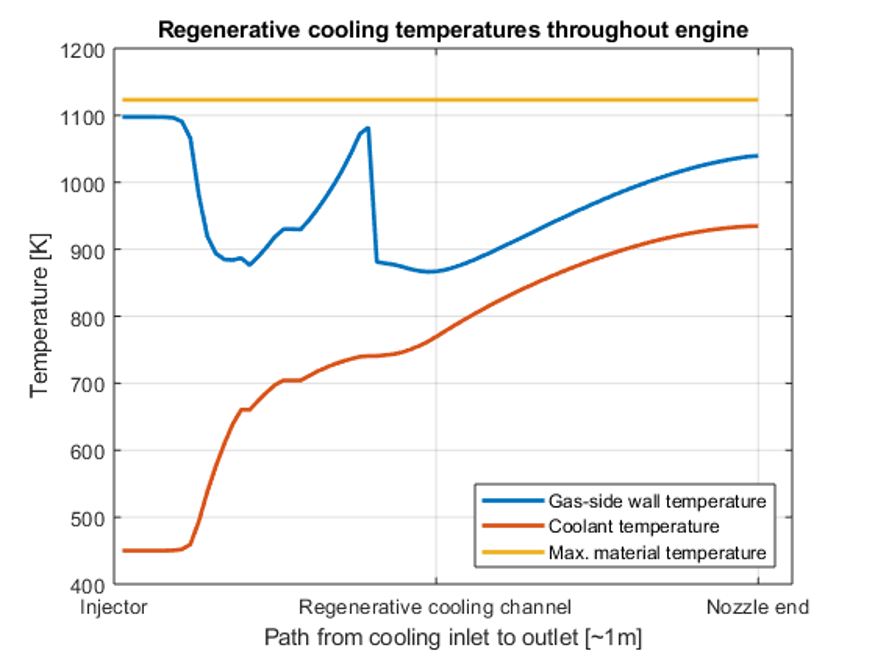
\includegraphics[width=0.9\linewidth]{relevanttemps}
	\caption{Regenerative cooling simulation - Relevant temperatures}\label{fig5}
\end{figure}

The highest temperatures can be observed in the combustion chamber section, as low flow speeds cause less convective heat transfer to take place, reducing the overall heat flux. The gas-side wall temperature then drops in the beginning of the throat area, before rising again towards the throat. After passing the throat, the gas-side wall temperature drops sharply and then rises again towards the nozzle exit.
\section{Hydrogen peroxide decomposition simulation}
\label{sec:11-3}
\qquad As mentioned in \autoref{sec:10-3}, the decomposition of hydrogen peroxide is used for self-pressurization of the oxidizer tank as well as power generation in a fuel cell in combination with hydrogen. As hydrogen peroxide is not only decomposing, but the decomposition is also an exothermal process, the thermal control system needs to be well under control in order to avoid critical behavior of the hydrogen peroxide if $150^\circ$ C are exceeded. Therefore, a detailed simulation has been performed, taking wall thicknesses, materials, radiative and absorbing coefficients as input parameters. The simulation is structured like a control system, calculating the temperature of the hydrogen peroxide inside the tank, the cold and hot wall temperatures. Upon reaching the specified target temperature, the control loop rotates the spacecraft to a neutral degree for constant hydrogen peroxide temperature. Before discussing the results, an overview of the simplifications taken for facilitation of the simulation follows:
\begin{itemize}
	\itemsep0em 
	\item	Inside the tank, only vaporization takes place, no condensation
	\item	The space craft can rotate to any angle instantaneously and there is no modelling of the necessary thruster activation
	\item	The cold and hot walls are always at a homogenous temperature, only depending on heat flux between hydrogen peroxide, the walls, the sun and dark space
	\item	As the structural calculations needed to be complete before the simulation was able to prove the technical feasibility of the decomposition regulation, \textbf{the hydrogen peroxide tank is assumed to be made of only one material throughout the rest of the documentation, while the simulation allows for two different materials}, as different heat flux coefficients are advantageous. Therefore, the results of this simulation are not exactly compatible with the final space craft design and more of a proof of concept, to be reunited with the structural design as a next step.
\end{itemize}

The simulation showed that, with the simplifications taken, a control system maintaining the hydrogen peroxide pressure at an acceptable level is technically feasible. A control reaction to raising the temperature from $310$ K to $350$ K has been chosen as the case for technical feasibility demonstration. As explained in \autoref{sec:10-3}, the rotational angle of the space craft is the dictating parameter for heat input and output. \autoref{fig6} shows the rotational angle, resulting H2O2 pressure, the relevant temperatures and the generated energy considering consumption of all generated oxygen in the fuel cell. The four graphs are outputs of the same simulation, the complete script and model for which can be found in the annex. The initial values for the integration blocks, which output temperatures, are all assumed.

\begin{figure}[H]
	\centering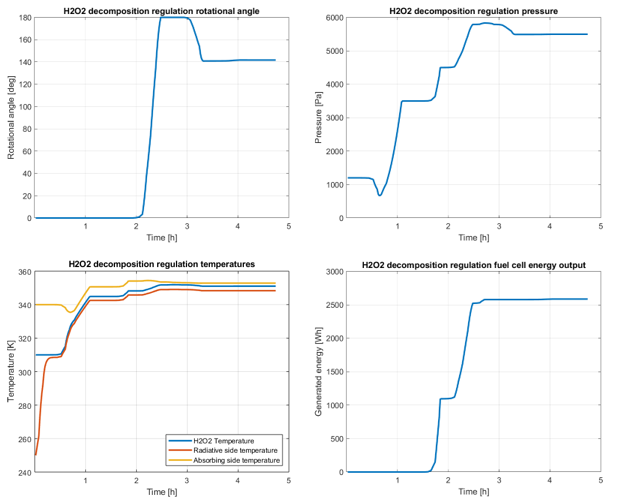
\includegraphics[width=\linewidth]{feasibility}
	\caption{Demonstration case for technical feasibility of $H_2O_2$ decomposition regulation}\label{fig6}
\end{figure}
As the simulation results show, the rotational angle is initially maintained at $0^\circ$, meaning full exposure of the more absorbing side towards the sun, with the less radiative side facing dark space. After $2$ hours, the space craft turns towards the other side, decreasing the heat flux gradually while approaching the target temperature. In the end, a constant neutral rotational angle of $140^\circ$ is maintained, with a final control error of around $1-2$ K. After this process, $2,5$ kWh of energy were generated, while the pressure inside the tank has risen from around $1000$ Pa to $5500$ Pa. The tank pressure is determined via interpolation of temperature-dependent vaporization pressures to gain a function of pressure with respect to temperature.
\chapter*{Conclusion}
\appendix




%\glsaddall
%\printglossaries

%\nocite{*}

	
%	\bibliographystyle{plain} % Le style est mis entre accolades.
%	\bibliography{references} % mon fichier de base de données s'appelle bibli.bib

%\printbibliography


\begin{acronym}[EHPAD] % Give the longest acronym here

\end{acronym}

\include{lexique_an_fr}
\listoffigures

\listoftables
\nopagebreak
\chapter*{Annexes}
\section*{Annex I - Gantt Diagramm}
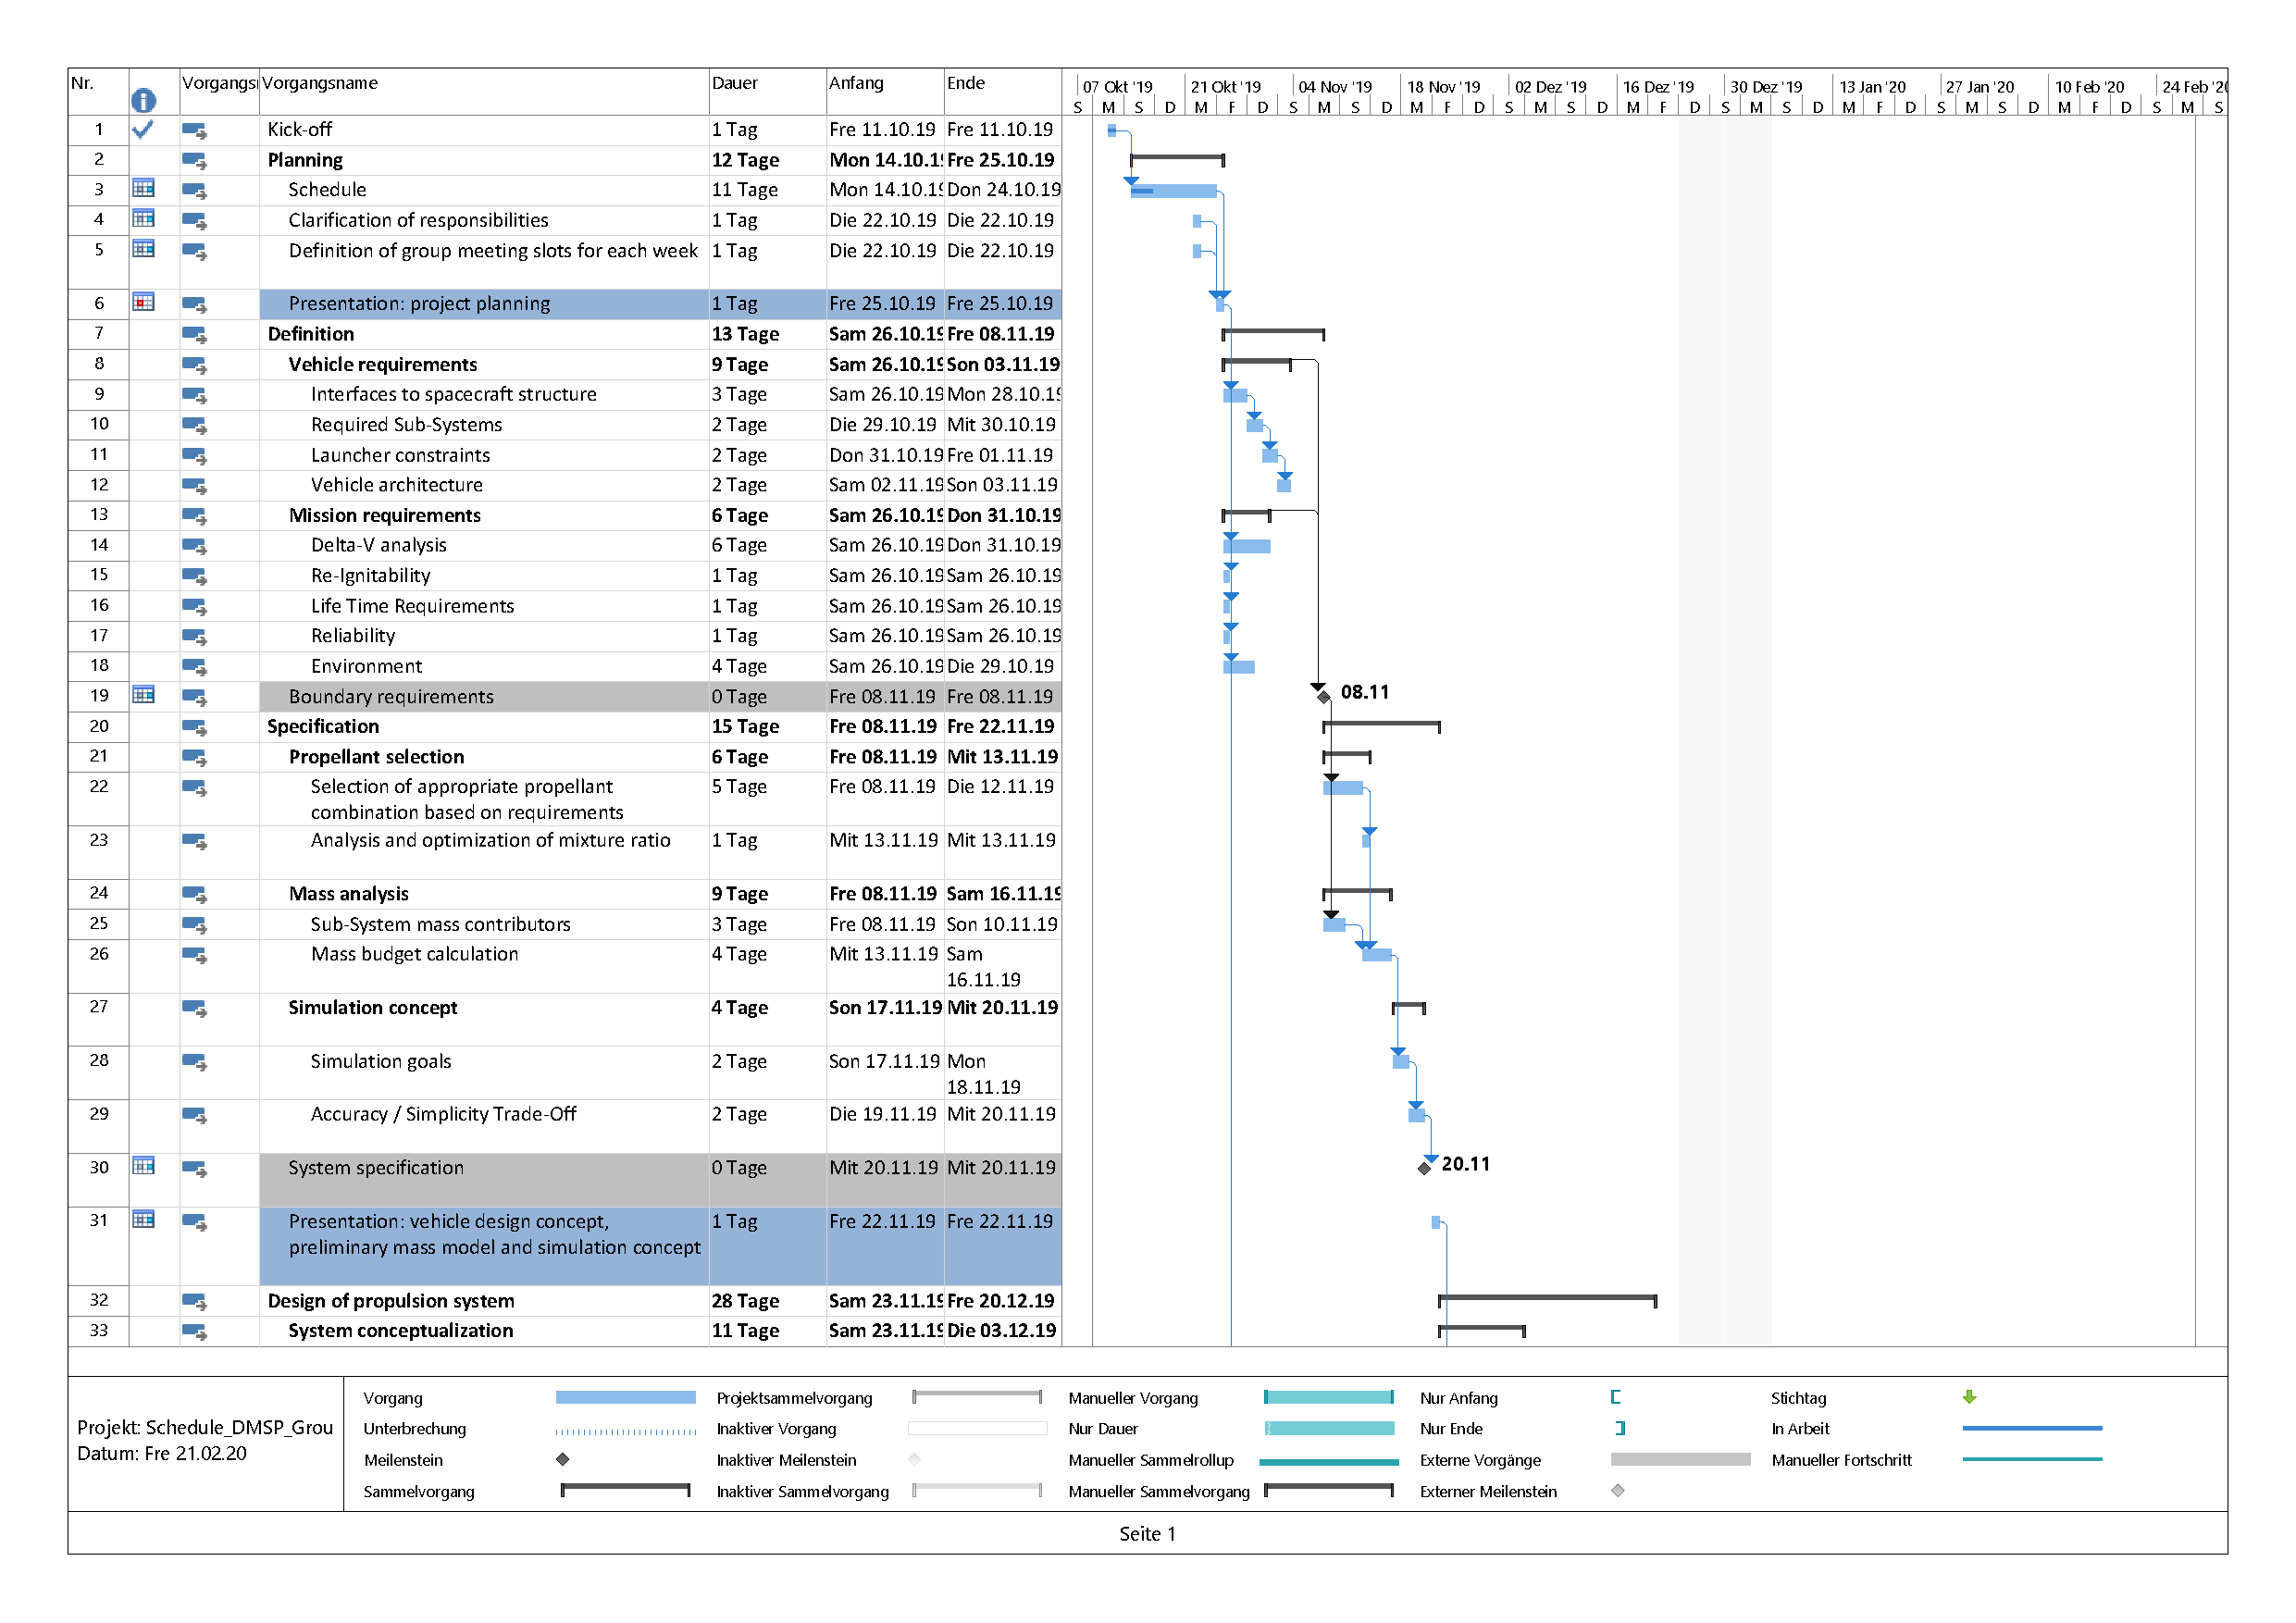
\includepdf[pages=-]{Gantt}\label{Gantt}


\printindex

\end{document}